\documentclass[12pt]{article} 
\usepackage[margin=1in]{geometry}
\usepackage{enumitem} %% for custom list
\usepackage{graphicx} %% for images
%\usepackage{multirow} %% for tables
%\usepackage{bigints}  %% for integrals
\usepackage[T1]{fontenc} %% for pipe simbol
\usepackage{amssymb}
\usepackage{amsmath}

% used for tabbed spacing
%\newcommand{\itab}[1]{\hspace{0em}\rlap{#1}}
%\newcommand{\tab}[1]{\hspace{.4\textwidth}\rlap{#1}}

\begin{document}
\date{}
%\author{Andrea Ghizzoni \\
%some other info}
\title{\vspace{-11ex}} %% used for no title
 
\maketitle
 
\section{Introduzione}\label{intro}
Nel corso del ventesimo secolo la tecnologia chiave \'e stata la raccolta, l'elaborazione e la distribuzione 
dell'informazione. Alcuni principali sviluppi a cui abbiamo assistito sono la costruzione di una rete telefonica mondiale, 
l'invenzione della radio e della televisione, la nascita e la crescita senza precedenti dell'industria informatica, il 
lancio dei satelliti per le telecomunicazioni e l'avvento di Internet.

Bench\'e  l'industria informatica sia ancora giovane a confronto di altre, come quelle automobilistica e dei trasporti
aerei, i computer hanno compiuto progressi spettacolari in breve tempo.

Nei primi due decenni della loro esistenza i sistemi informatici erano altamente centralizzati; una azienda di medie
dimensioni o un'universit\'a potevano disporre di uno o due computer, mentre le grandi istituzioni ne possedevano al 
massimo una dozzina.

Il concetto un tempo dominante di \textit{centro di calcolo} come una stanza con un grande computer dove gli utenti 
portavano il loro lavoro per l'elaborazione oggi \'e completamente superato, sostituito da un modello in cui il lavoro \'e 
svolto da un gran numero di computer distinti, ma connessi. Questi sistemi sono chiamati \textbf{reti di calcolatori}.

Per reti di calcolatori si intende un insieme di computer autonomi connessi ad una singola tecnologia. Due computer si
dicono connessi quando sono in grado di scambiare informazioni.

Le reti hanno dimensioni, topologie e caratteristiche differenti e vengono solitamente connesse fra di loro per formare
reti pi\'u grandi fino ad arrivare ad \textbf{Internet} che \'e il pi\'u famoso esempio di reti di reti.

\paragraph{Sistemi Distribuiti} Un sistema distribuito \'e un insieme di computer, indipendenti tra di loro, che appare
all'utente come un singolo sistema coerente, presentato solitamente a livello software (\textbf{middlware}). L'esempio 
pi\'u classico \'e il \textbf{World Wide Web}.

\paragraph{Reti di Calcolatori} Una rete di calcolatori \'e un insieme di computer ma dal punto di vista utente percepiti
come macchine effettive, con hardware e sistemi operativi differenti. Per l'utilizzo di un particolare applicativo \'e
necessario individuare la macchina su cui risiede, connettersi ad essa e solo a quel punto eseguirlo.

\clearpage
\subsection{Applicazioni Aziendali}\label{applicazioni-aziendali}
L'uso principale delle infrastrutture di rete a livello aziendale \'e la condivisione di risorse, programmi e periferiche 
senza doverne specificare l'ubicazione fisica. Un esempio ovvio \'e riguarda la necessit\'a di condividere una stampante.

Si pu\'o immaginare il sistema informatico di un'azienda come formato da uno o pi\'u database e da un certo numero di
impiegati che hanno bisogno di accedervi da remoto. In questo modello i dati sono memorizzati in computer ad alte
prestazioni chiamati \textbf{server}, mentre gli impiegati dispongono di macchine pi\'u semplici chiamate 
\textbf{client}.

Questa configurazione \textbf{client-server}, \'e ampiamente utilizzata e rappresenta il punto di partenza di 
gran parte dell'utilizzo delle reti. L'utilizzo pi\'u noto \'e quella di \textbf{un'applicazione Web}, in cui il 
server genera dei contenuti in risposta ad una richiesta da parte del client.

Una variante di questo modello di accesso alle informazioni prende il nome di \textbf{peer-to-peer}, nel quale ogni 
entit\'a pu\'o comunicare con qualsiasi altra entit\'a all'interno del gruppo di computer, senza che ci sia una 
distinzione netta tra client e server. In questo caso non esiste alcun "database" centralizzato dei contenuti, invece ogni 
utente mantiene le informazioni in locale, permettendo agli altri utenti a lui noti che fanno parte del sistema di consultarle.

\subsection{Applicazioni Domestiche}\label{applicazioni-domestiche}
Il principale utilizzo di un personal computer nell'ambito domestico \'e l'accesso a Internet.


\clearpage
\section{Astrazione di una Rete di Computers}\label{astrazione-di-una-rete-di-computers}
Concettualmente una rete di computer pu\'o essere vista come un \textit{Grafo}, da cui le seguenti definizioni:
\begin{quote}
	\textit{Una rete di computer \'e un insieme di nodi e canali con lo scopo di fornire un collegamento tra due o pi\'u punti
	per permettere la telecomunicazione tra essi.}
\end{quote}

\begin{quote}
	\textit{Si definisce nodo un punto in cui avviene la commutazione o l'elaborazione dell'informazione.}
\end{quote}

\begin{quote}
	\textit{Si definisce canale un mezzo di trasmissione oppure un collegamento logico, realizzato tramite diverse tecnologie di 
	trasmissione.}
\end{quote}
Pi\'u formalmente si definisce un grafo come:
\begin{center}
	\textbf{G=(V,A)}
\end{center}
dove
\begin{itemize}[noitemsep]
	\item V := insieme dei vertici o nodi della rete
	\item A := insieme degli archi o dei collegamenti/canali di comunicazione
\end{itemize}
Gli archi possono essere \textbf{non-diretti} o \textbf{diretti}, per permettere la comunicazione in uno o entrambi i
sensi. 

\'E possibile definire ulteriormente:
\begin{itemize}[noitemsep]
	\item N := |V| come numero di vertici/nodi
	\item C := |C| come numero di archi/canali 
\end{itemize}

\paragraph{In Sintesi:}
L'astrazione di una rete di computer in un grafo ci aiuta nella progettazione e nell'analisi dei costi generali, ma per la 
costruzione pratica \'e necessario specificare: : \textit{il tipo di collegamento} e \textit1{la scala}, ovvero come 
dovranno essere realizzati ogni collegamento dei nodi e le dimensioni finali della rete e di ogni collegamento.


\clearpage
\section{Tipologia di Collegamenti}\label{tipologia-di-collegamenti}
Di seguito sono riportati le vari modalit\'a di collegamenti tra computer che si possono trovare in una rete di 
comunicazione.

\subsection{Collegamenti Punto-Punto}\label{collegamenti-punto-punto}
\begin{center}
	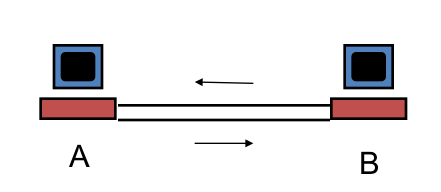
\includegraphics[scale=0.5]{introduzione-img1.png}
\end{center}
I collegamenti Punto-Punto sono la forma pi\'u comune di collegamento in quanto connettono coppie di computer. Il 
collegamento pu\'o avvenire anche se prevede delle macchine intermedie. Nel caso in cui ci sia solo un trasmettitore e un 
ricevitore viene chiamata anche \textbf{unicast}.

\subsection{Collegamenti Multi-Punto o Broadcast}\label{collegamenti-multi-punto-broadcast}
\begin{center}
	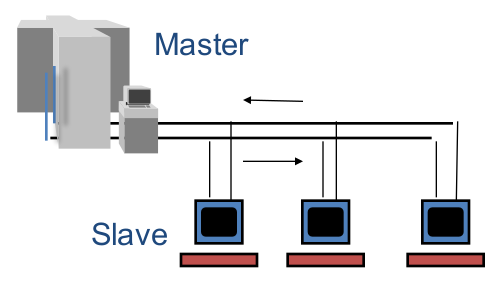
\includegraphics[scale=0.5]{introduzione-img2.png}
	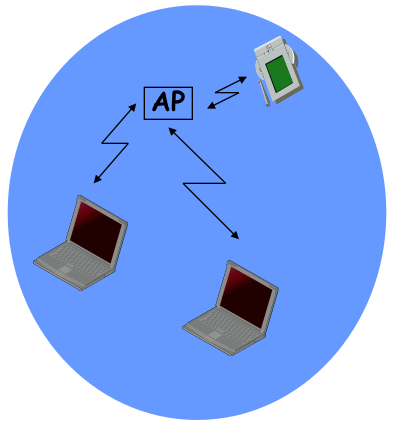
\includegraphics[scale=0.35]{introduzione-img3.png}
\end{center}
Al contrario delle reti punto-punto, le reti multi-punto o broadcast hanno un solo canale di comunicazione condiviso da 
tutte le macchine della rete. I messaggi inviati da qualunque macchina sono ricevuti da tutte le altre. Un campo indirizzo 
all'interno del messaggio individua il destinatario. Se il messaggio \'e indirizzato alla macchina ricevente allora viene
processato, altrimenti viene ignorato.

Un esempio di rete multi-punto \'e il bus di trasferimento dati usato in tutti i calcolatori: quando il processore inizia a 
trasmettere dati con una periferica (viste come computer sulla rete), le altre sentono il bus occupato e non iniziano una 
trasmissione a loro volta, ma solo quando il processore consente loro di farlo.

Un secondo esempio \'e la classica rete wireless, dove ci sono molti dispositivi con capacit\'a di trasmettere e ricevere
attraverso onde elettromagnetiche. In questo caso il mezzo di trasmissione condiviso \'e l'etere.


\section{Topologia delle Reti}\label{topologia-delle-reti}
Come visto nella sezione \ref{astrazione-di-una-rete-di-computers}, \'e possibile interpretare una rete di computer come un 
grafo. In questo modo nascono diverse topologie:

\subsection{Maglia Completa}\label{maglia-completa}
\begin{center}
	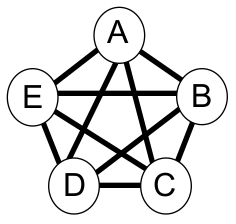
\includegraphics[scale=0.5]{introduzione-img4.png}
\end{center}
Questa topologia prevede che tutti i nodi siano collegati con tutti gli altri nodi, creando cos\'i una maglia di collegamenti, da 
cui il nome maglia completa.
\begin{itemize}[noitemsep]
	\item \textbf{Vantaggi:}
	\begin{itemize}[noitemsep]
		\item Alta tolleranza ai guasti, grazie a collegamenti ridondanti
		\item Banali algoritmi per gestire l'inoltro dei messaggi
	\end{itemize}
	\item \textbf{Svantaggi:}
	\begin{itemize}[noitemsep]
		\item L'alto numero di collegamenti la rende poco attuabile quando il numero di nodi inizia a crescere
	\end{itemize}
\end{itemize}

\subsection{Maglia o Mesh}\label{mesh}
\begin{center}
	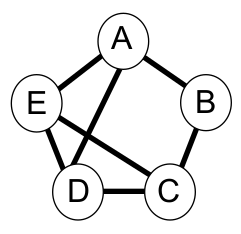
\includegraphics[scale=0.5]{introduzione-img7.png}
\end{center}
In questo caso abbiamo una topologia molto simile alla maglia completa ma si riducono il numero di collegamenti tra i nodi.
\'E tutt'ora la base di Internet e del sistema telefonico.
\begin{itemize}[noitemsep]
	\item \textbf{Vantaggi:}
	\begin{itemize}[noitemsep]
		\item Costi contenuti grazie al numero di canali selezionabili a piacere
	\end{itemize}
	\item \textbf{Svantaggi:}
	\begin{itemize}[noitemsep]
		\item Una pi\'u complessa gestione di inoltro dei messaggi
	\end{itemize}
\end{itemize}

\subsection{Albero}\label{albero}
\begin{center}
	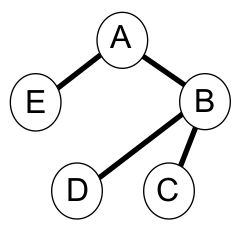
\includegraphics[scale=0.5]{introduzione-img5.png}
\end{center}
La topologia ad albero prevede che i nodi siano strutturati in modo gerarchico, identificando un nodo radice ed i suoi 
figli. Viene molto usata ancora oggi come topologia logica invece che fisica; questo porta il vantaggio di ragionare 
sulla topologia ad albero, ma in realt\'a l'effettiva rete fisica pu\'o essere una a maglia.
\begin{itemize}[noitemsep]
	\item \textbf{Vantaggi:}
	\begin{itemize}[noitemsep]
		\item Costi contenuti causa il basso numero di canali
		\item Algoritmi di inoltro dei messaggi molto semplici
	\end{itemize}
	\item \textbf{Svantaggi:}
	\begin{itemize}[noitemsep]
		\item Alta vulnerabilit\'a ai guasti, perch\'e esiste un solo canale tra due nodi
	\end{itemize}
\end{itemize}

\subsection{Stella}\label{stella}
\begin{center}
	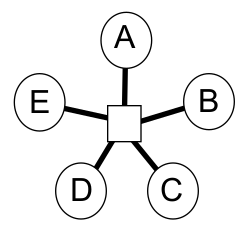
\includegraphics[scale=0.5]{introduzione-img6.png}
\end{center}
La topologia a stella veniva molto usata agli albori delle reti di calcolatori, quando esisteva un grosso calcolatore 
aziendale che eseguiva i programmi degli utenti collegati tramite terminali.

Attualmente troviamo questa topologia tipicamente nelle reti domestiche, cellulari e satellitari.
\begin{itemize}[noitemsep]
	\item \textbf{Vantaggi:}
	\begin{itemize}[noitemsep]
		\item Basso numero di canali: uno per nodo
		\item Semplifica la stesura dei canali
	\end{itemize}
	\item \textbf{Svantaggi:}
	\begin{itemize}[noitemsep]
		\item Tutta la complessit\'a dell'inoltro dei messaggi risiede nel centro stella, ogni nodo comunica solo col centro
		      stella
		\item Vulnerabilit\'a ai guasti del centro stella
	\end{itemize}
\end{itemize}

\subsection{Anello}\label{anello}
\begin{center}
	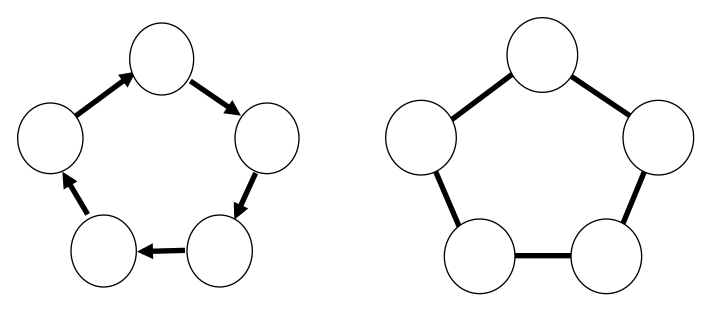
\includegraphics[scale=0.36]{introduzione-img8.png}
\end{center}
La topologia ad anello veniva usata nelle prime reti locali e tutt'oggi nelle reti metropolitane. Il principio di 
funzionamento \'e molto semplice: si costruisce un anello unidirezionale o bidirezionale nel quale ogni nodo pu\'o 
comunicare solo col proprio successivo nell'anello.

Una tecnica costruttiva per aumentare la ridondanza di canali in questo tipo di topologia \'e quella di costruire pi\'u reti 
ad anello sovrapposti.
\begin{itemize}[noitemsep]
	\item \textbf{Vantaggi:}
	\begin{itemize}[noitemsep]
		\item Tolleranza al guasto di un canale (anello bidirezionale)
		\item Inoltro dei messaggi molto semplice
		\item Basso numero di canali
	\end{itemize}
	\item \textbf{Svantaggi:}
	\begin{itemize}[noitemsep]
		\item Con anello unidirezionale in caso di guasti multipli possono rimanere isolati dei nodi
	\end{itemize}
\end{itemize}

\subsection{Bus}\label{bus}
\begin{center}
	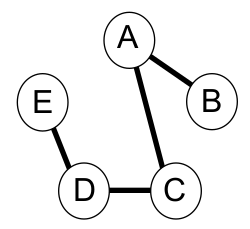
\includegraphics[scale=0.5]{introduzione-img9.png}
\end{center}
Questo tipo di topologia veniva usato nelle reti locali, quando il collegamento tra i nodi della rete era molto costoso.
Ogni nodo veniva collegato ad un canale condiviso, detto bus, per permettere la comunicazione con tutta la rete.
\begin{itemize}[noitemsep]
	\item \textbf{Vantaggi:}
	\begin{itemize}[noitemsep]
		\item Bassi costi di realizzazione: usa il numero minimo di canali
		\item Algoritmi di inoltro dei messaggi molto semplici: esiste un solo percorso tra due coppie di nodi
	\end{itemize}
	\item \textbf{Svantaggi:}
	\begin{itemize}[noitemsep]
		\item Bassissima tolleranza ai guasti
	\end{itemize}
\end{itemize}


\section{Protocollo}\label{protocollo}
Dopo aver definito come una rete si formalizza con la teoria dei grafi (sezione \ref{astrazione-di-una-rete-di-computers}) e
come si realizzano i collegamenti (sezione \ref{tipologia-di-collegamenti}) \'e necessario definire come le informazioni
vengono effettivamente trasmesse. \'E necessario definire dei \textbf{protocolli di comunicazione} in modo da avere un insieme 
di regole comuni tra tutti i dispositivi di rete, al fine che l'informazione venga trasmessa e ricevuta correttamente.

\subsection{Definizione}\label{definizione}
\begin{quote}
    \textit{Un protocollo definisce il formato e l'ordine dei messaggi scambiati tra due o pi\'u	entit\'a in comunicazione, 
    cos\'i come le azioni da intraprese in fase di trasmissione e/o ricezione di un messaggio o di un altro evento}
\end{quote}
Un'entit\'a pu\'o essere formalizzata come un processo in esecuzione su un calcolatore che riesce a comunicare un messaggio 
tramite un determinato protocollo.
\begin{center}
	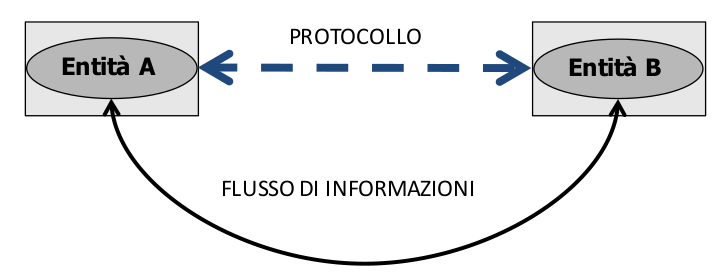
\includegraphics[scale=0.4]{introduzione-img10.png}
\end{center}
\paragraph{Protocollo $\neq$ Linguaggio di Programmazione} Molte volte si confonde il termine protocollo con quello di 
linguaggio di programmazione: il protocollo \'e un insieme di regole che permettono la comunicazione tra entit\'a diverse, 
mentre il linguaggio di programmazione permette l'esecuzione di calcoli aritmetici al un calcolatore. 

Tra le due definizioni \'e possibile fare molta confusione perch\'e hanno alcune caratteristiche comuni, ma la differenza 
sostanziale sta nell'elaborazione delle informazioni: le reti di comunicazioni non computano nulla, permettono solo la 
trasmissioni di dati, mentre il linguaggio di programmazione pu\'o computare un informazione e trasmetterla attraverso la rete 
usando determinati protocolli.

\paragraph{Internet \'e un protocollo? No!} Molti confondono Internet come un protocollo, ma in realt\'a non sono oggetti
confrontabili, perch\'e i protocollo sono un insieme di regole, mentre internet \'e una rete di reti.

\clearpage
%%\subsection{Componenti}\label{componenti}
%%Per definire un protocollo di comunicazione sono necessari:
%%\begin{itemize}[noitemsep]
%%    \item \underline{Sintassi}: insieme dei formati che consentono il riconoscimento dei messaggi
%%    \item \underline{Semantica}: algoritmi che definiscono il funzionamento del protocollo
%%    \item \underline{Temporizzazione}: logica temporale di funzionamento di un protocollo
%%\end{itemize}

\subsection{Architettura Protocollare}\label{architettura-protocollare}
Per il corretto funzionamento delle reti di calcolatori sono necessari diversi protocolli: da quelli utilizzati nelle 
applicazioni, a quelli che definiscono i metodi di trasferimento sul mezzo fisico. Ognuno di questi si pu\'o formalizzare come 
un livello logico, concettualmente separato dagli altri. 

Per la progettazione di ogni livello \'e stato usato un sistema \textit{stratificato}, ovvero: ogni livello implementa le 
proprie funzioni di protocollo e svolge servizi per i livelli superiori.

L'insieme di tutti i livelli logici cosi definiti viene chiamato \textbf{Architettura Protocollare} o \textbf{Pila 
Protocollare}.

Il motivo principale dell'utilizzo di una architettura stratificata \'e la separazione logica dei vari livelli, che comporta
l'implementazione separata di ogni singolo livello, con notevoli vantaggi al programmatore. Sotto certi aspetti \'e molto
simile al sviluppo modulare di un qualsiasi applicativo: pezzi riutilizzabili, librerie senza dipendenze esterne, costruzione 
funzionale dei servizi ecc...

Ogni livello \'e progettato, nel caso di invio di messaggi, in modo tale da ricevere informazioni dal livello 
superiore, elaborarle e passarle al livello sottostante. Nella ricezione di messaggi, invece, ricever\'a informazioni dal 
livello sottostante e, una volta elaborate, le trasferir\'a al livello superiore.

Inoltre, ad ogni livello, vengono aggiunte delle informazioni di controllo all'inizio e alla fine del messaggio, chiamati 
\textbf{Header} e \textbf{Trailer} o congiuntamente \textbf{PCI} \textit{(Protocol Control Interface)}. Questa tecnica viene 
chiamata \textbf{Incapsulamento}. L'intero processo \'e mostrato nella figura successiva insieme ad una anticipazione del modello 
ISO/OSI che verr\'a spiegato nella sezione successiva:
\begin{center}
	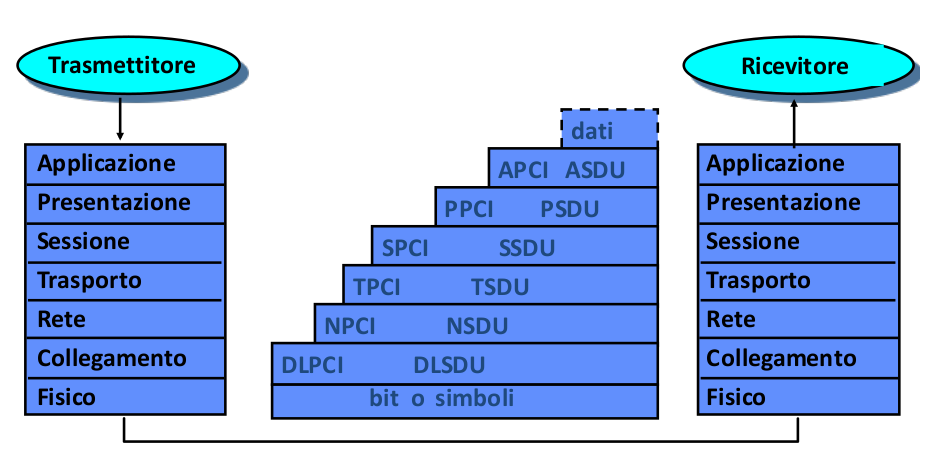
\includegraphics[scale=0.4]{introduzione-img13.png}
\end{center}
Come si nota dall'immagine precedente, ad ogni livello l'informazione prende dei nomi diversi: \textit{ASDU, PSDU..}
In generale si pu\'o definire: 
\begin{itemize}[noitemsep]
    \item \textbf{PDU} \textit{(Protocol Data Unit)} come l'informazione ricevuta dal livello superiore/inferiore ancora non 
    elaborata
    \item \textbf{SDU} \textit{(Service Data Unit)} come PDU + PCI
    \item \textbf{SAP} \textit{(Service Access Point)} come il punto di accesso al servizio di livello superiore/inferiore
\end{itemize}
L'intero processo \'e schematizzato come segue:
\begin{center}
	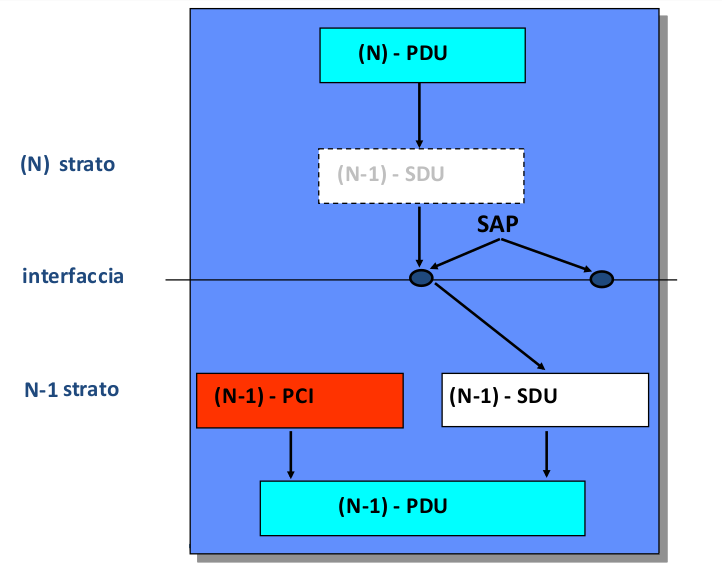
\includegraphics[scale=0.4]{introduzione-img12.png}
\end{center}
Da notare che il solo modo che ha il livello N di comunicare con il livello N$\pm$1 \'e attraverso le SAP, quindi nel caso ci 
dovessero essere dei cambiamenti di logica al livello N$\pm$1, non intaccherebbe il livello N, in quanto l'interfaccia di 
collegamento non viene modificata.

\subsection{Il Modello ISO/OSI}\label{il-modello-iso-osi}
L'architettura protocollare utilizzata in internet \'e chiamata \textbf{modello ISO/OSI} (International Organization for 
Standardization/Open System Interconnection) e definisce i 7 livelli protocollari mostrati in figura:
\begin{center}
	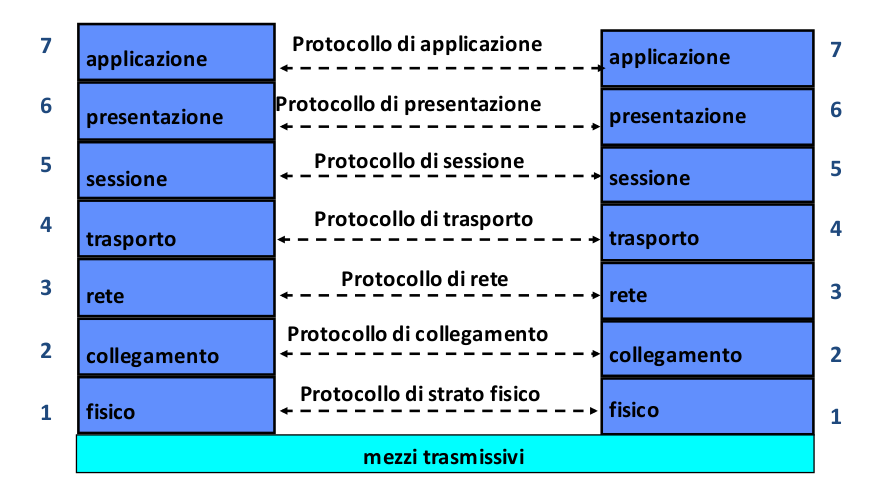
\includegraphics[scale=0.35]{introduzione-img11.png}
\end{center}
Notare che nella figura precedente si rispetta la definizione di protocollo tra entit\'a: il un entit\'a a livello applicazione
comunica con un'altra enti\'a di livello applicazione tramite il protocollo di applicazione.

\subsubsection{ISO/OSI in breve}\label{iso-osi-in-breve}
\begin{itemize}
	\item \textbf{Il livello Fisico:} il livello fisico si occupa della trasmissione dei bit grezzi sul canale di 
    comunicazione. Problemi tipici riguardano quali segnali elettrici dovrebbero essere usati per rappresentare un 1 o uno 
    0, quanti nanosecondi deve durare un bit, se la trasmissione pu\'o avvenire simultaneamente in entrambe le direzioni, 
    come si stabilisce la connessione iniziale e come viene abbattuta quando entrambe le parti hanno terminato, quanti contatti 
    deve avere il connettore di rete e quale funzione va assegnata a ciascuno.
    
    \item \textbf{Il livello Collegamento:} il compito principale del livello di collegamento consiste nel far diventare una 
    trasmissione grezza in una linea che appare priva di errori non rilevanti. Quindi maschera gli errori in modo che il livello 
    di rete non li veda. L'obiettivo \'e raggiunto forzando la sorgente a suddividere i dati in ingresso, chiamati \textbf{frame}, 
    trasmessi sequenzialmente. 
    
    Un altro problema che nasce nel livello collegamento riguarda il modo di evitare che un trasmittente veloce saturi il buffer 
    di un ricevente lento; occorre quindi un meccanismo per regolare il traffico. 
    
    Le reti broadcast hanno un problema in pi\'u nel livello collegamento: come controllare l'accesso al canale condiviso. Di 
    questo problema si occupa uno speciale sottoinsieme del livello collegamento chiamato \textbf{MAC} \textit{(Medium Access 
    Control)}.
    
    \item \textbf{Il livello di Rete:} il livello di rete controlla il funzionamento della sottorete. Un problema chiave riguarda
    la modalit\'a con cui i pacchetti sono inoltrati dalla sorgente alla destinazione. I percorsi lungo i quali effettuare 
    l'inoltro possono essere statici o, pi\'u spesso, vengono calcolati e aggiornati automaticamente. 
    
    Un secondo problema \'e quello di coni di bottiglia causati dalla impossibilit\'a di inoltro a causa di troppi pacchetti. Il 
    controllo di queste congestioni spetta al livello di rete in collaborazione con i livelli pi\'u alti che si adattano al carico 
    della rete. Pi\'u in generale, la qualit\'a del servizio offerto (ritardo, tempo di transito, jitter ecc) \'e un problema del 
    livello di rete. 
    
    Quando un pacchetto deve viaggiare da una rete all'altra per arrivare a destinazione possono nascere dei problemi: 
    indirizzamento, rifiuto del pacchetto perch\'e troppo grande, protocolli diversi ecc. \'E compito del livello di rete 
    risolvere questi problemi per consentire la comunicazione tra reti diverse.
    
    \clearpage
    \item \textbf{Il livello Trasporto:} la funzione essenziale del livello trasporto \'e quella di accettare dati dal livello 
    superiore, dividerli il unit\'a pi\'u piccole quando necessario, passarle al livello di rete e assicurarsi che tutti i pezzi 
    arrivino correttamente a destinazione. Stabilisce che tipo di servizio offrire agli utenti della rete durante l'instaurarsi della 
    connessione. 
    
    Il livello trasporto copre tutto il percorso tra sorgente e destinazione; in 
    altri termini, un programma sul computer sorgente instaura una connessione con un programma corrispondente sul computer 
    destinatario, utilizzando intestazioni dei messaggi e messaggi di controllo. Nei livelli inferiori i protocolli riguardano la 
    comunicazione tra ciascun computer e i vicini immediati, e non tra i computer sorgente e destinazione, che possono essere 
    separati da router. Il livello trasporto definisce, quindi, \textbf{protocolli end-to-end}.
    
    \item \textbf{Il livello Sessione:} il livello sessione permette a utenti su computer diversi di stabilire tra loro una 
    sessione, che permettono tra cui: controllo del dialogo, gestione dei token e sincronizzazione.
    
    \item \textbf{Il livello Presentazione:} il livello presentazione si occupa della sintassi e della semantica dell'informazione 
    trasmessa. Per consentire la comunicazione con differenti rappresentazioni dei dati il livello presentazione definisce strutture 
    dati astratte che consentono lo scambio e la definizione di strutture dati di livello superiore.
    
    \item \textbf{Il livello Applicazione:} il livello applicazione compre una variet\'a di protocolli comunemente richiesti dagli 
    utenti. Un protocollo applicativo largamente usato e' \textbf{HTTP} \textit{(Hyper Text Transfer Protocol)}, la base del World 
    Wide Web.    
\end{itemize}

\clearpage
\subsection{Relay System}\label{relay-system}
Il modello ISO/OSI non obbliga tutti i calcolatori ad implementare tutti i livelli definiti dallo standard. Esistono apparati 
di rete che implementano solo i primi 2 livelli, chiamati \textit{Switch} mentre ne esistono altri che implementano solo i 
primi 3, chiamati \textit{Router}.
\begin{center}
	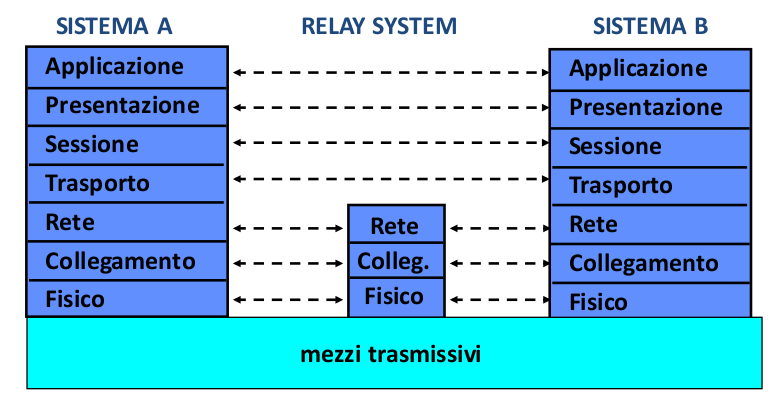
\includegraphics[scale=0.45]{introduzione-img14.png}
\end{center}
I Router e gli Switch vengono chiamati anche \textit{Relay System}.

\subsection{Riassumendo}\label{riassumendo}
Nell'immagine seguente vengono riassunti tutti i concetti e le tecniche illustrate in questa sezione
\begin{center}
	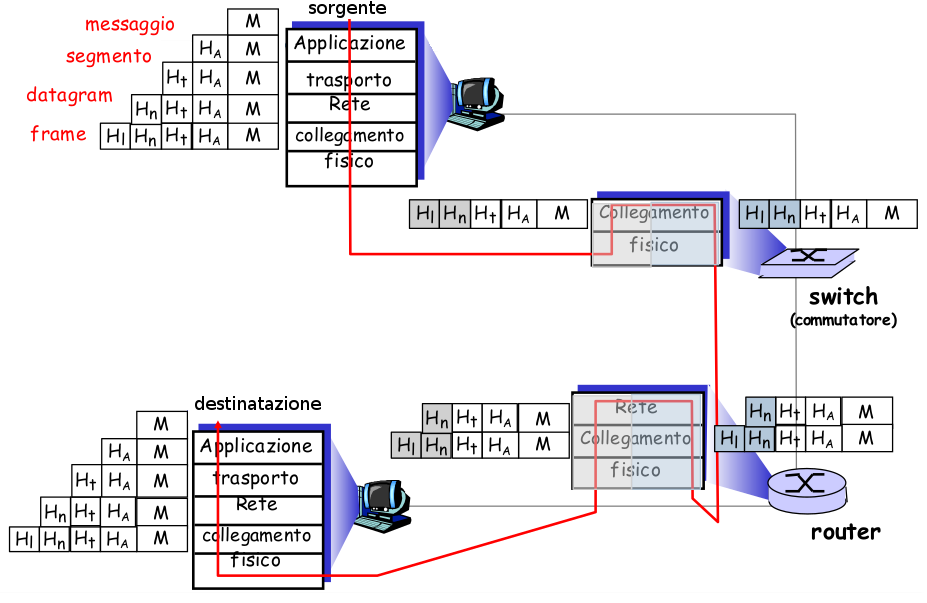
\includegraphics[scale=0.5]{introduzione-img15.png}
\end{center}


\clearpage
\section{Internet: una panoramica contestualizzata}\label{internet-una-panoramica-contestualizzata}
Internet \'e una collezione di reti diverse che usano protocolli comuni per la comunicazione e per l'offerta di servizi. 

La rete internet deve occuparsi \underline{solo} del trasporto delle informazioni. L'analisi e l'elaborazione dovrebbe essere svolta 
solo dagli host ai confini della rete. Purtroppo questo non e' pi\' vero a causa dei \textit{Firewall}.

\'E un sistema inconsueto che non ha un progettista e non \'e controllato da nessuno. 

\subsection{La Storia}\label{la-storia-di-internet}
\subsubsection{ARPANET}\label{arpanet}
Nel pieno della guerra fredda, il dipartimento della difesa USA commissiona una rete di controllo che possa sopravvivere 
a una guerra nucleare. All'epoca, essendo che tutte le comunicazioni militari usavano la rete telefonica pubblica, venne 
considerata troppo vulnerabile di attacchi mirati ad alcune infrastrutture, in quando realizzata in modo gerarchico, dove
esisteva una centrale che connetteva centinaia di altre centrali, che a sua volta connetteva migliaia di apparecchi.

Attorno al 1960, il dipartimento di difesa assegn\'o il compito di trovare una soluzione. Paul Baran svilupp\'o il progetto
di una rete altamente distribuita, resistente ai guasti e a distribuzione di pacchetto, quindi chiesero la realizzazione 
ad AT\&T, all'epoca detentore delle infrastrutture fisiche nel paese. Purtroppo si rifiutarono, rispondendo che era un progetto 
di impossibile realizzazione. Il progetto di Baran venne quindi abbandonato.

Nell'ottobre del 1957, l'Unione Sovietica batt\'e gli USA nella corsa alla conquista dello spazio, la risposta 
dell'allora presidente Eisenhower fu (tra le altre) quella della creazione di una singola organizzazione per la 
ricerca, \textbf{ARPA} \textit{(Advanced Research Projects Agency)}. ARPA non disponeva di scienziati o laboratori; in 
effetti non aveva altro che un ufficio e un piccolo budget. Il suo compito era di erogare fondi e stipulare contratti con 
universit\'a e aziende che avevano idee promettenti. 

Nel 1976 ARPA contatt\'o Wesly Clark, che sugger\'i di costruire una sottorete a commutazione di pacchetto, connettendo 
ogni host a un proprio router. Ogni sottorete sarebbe stata composta da un microcomputer chiamato \textbf{IMP} \textit{(Interface 
Message Processor)} collegati da linee di trasmissione a 56 kbps. Per raggiungere un'alta affidabilit\'a ogni IMP doveva essere 
collegato ad almeno altri due IMP, cos\'i in caso di distruzione di alcune linee o IMP i messaggi sarebbero stati automaticamente 
inoltrati su percorsi alternativi.

Ogni nodo della rete doveva consistere in un IMP e un host, il quale avrebbe potuto mandare messaggi con lunghezza massima di 8.063 
bit al suo IMP che li avrebbe suddivisi in pacchetti di massimo 1.008 bit per inoltrarli indipendentemente verso la destinazione.
La rete cos\'i progettata prese il nome di \textbf{ARPANET}.

ARPA band\'i una gara d'appalto per costruire la sottorete. Scelse BBN, una societ\'a di consulenza di Cambrige, Massachusetts, e 
nel dicembre 1968 le assegno l'appalto e il compito di scrivere il relativo software. BBN scelse come IMP dei minicomputer 
Honeywell DDP-316 appositamente modificati, con memoria a nuclei magnetici di 12 K organizzata in word di 16 bit, senza dischi, 
poich\'e le parti mobili erano considerate inaffidabili. Gli IMP erano collegati a linee affittate a 56 kbps. Il software della 
sottorete era composto dalla parte lato IMP, della connessione tra IMP e host, dal protocollo IMP-IMP e da un protocollo da IMP 
sorgente a IMP destinazione, progettato per migliorare l'affidabilit\'a.

Fuori dalla sottorete era necessario altro software, in particolare il lato host della connessione host-IMP, il protocollo host-host 
e il software applicativo. Per affrontare il problema, Clark organizz\'o a Snowbird, Utah, un incontro di ricercatori specializzati in 
reti di calcolatori.

In qualche modo una rete sperimentale entr\'o in servizio del dicembre 1969 con quattro nodi: UCLA, UCSB, SRI e Universit\'a dello 
Utah.
\begin{center}
	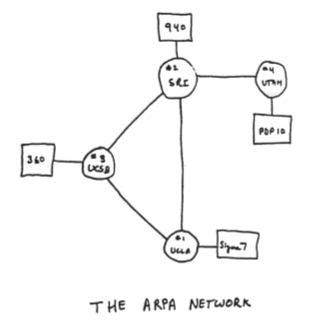
\includegraphics[scale=0.5]{introduzione-img16.png}
\end{center}
La rete crebbe man mano che altri IMP vennero consegnati ed installati; presto copr\'i tutti gli Stati Uniti.

\paragraph{Funny Story} Oltre ad aiutare la crescita di ARPANET, ARPA finanzi\'o ricerche sull'uso di reti satellitari e reti 
radiomobili a pacchetto. Durante una celebre dimostrazione, un camion in movimento situato in California us\'o la rete radiomobile a 
pacchetto per mandare messaggi a SRI, inoltrati su ARPANET fino alla costa Est, e quindi inviati alla University College di Londra 
tramite una rete satellitare. I ricercatori riuscirono ad usare un computer a Londra mentre si muovevano per la California.\\

Molti esperimenti dimostrarono che i protocolli esistenti di ARPANET non si potevano usare per reti multiple. Tale osservazione 
stimol\'o le ricerche sui protocolli, culminate con l'invenzione del modello TCP/IP. Questo protocollo fu specificatamente progettato 
per gestire la comunicazione sulle internet-work, che stavano crescendo d'importanza man mano che nuove reti venivano collegate ad 
ARPANET.

ARPA conosceva molti contatti a BBN e all'Universit\'a della California a Berkeley per integrarli nello UNIX di Berkeley. I 
ricercatori svilupparono una pratica interfaccia di programmazione verso la rete (socket) e scrissero molte applicazioni, utility e 
programmi di gestione per semplificare la connessione.

Quando usc\'i BSD 4.2 con TCP/IP, le socket e una montagna di utility per la rete, l'adozione dell'intero pacchetto fu immediata. 
Con TCP/IP diventava semplice collegare una LAN ad ARPANET, e molti lo fecero.

Nel corso degli anni '80, al crescere delle dimensioni della rete, rintracciare un host divent\'o sempre pi\'u difficoltoso, quindi 
fu creato il \textbf{DNS} \textit{(Domain Name System)} per organizzare i computer in domini e abbinare i nomi degli host agli 
indirizzi IP.

\subsubsection{NSFNET}\label{nsfnet}
L'NSF \textit{(National Science Foundation)}, si accorse dell'enorme impatto che ARPANET aveva sulla ricerca, permettendo a 
scienziati di tutto il paese di condividere i dati e collaborare a progetti di ricerca.

NSF decise di costruire una rete di dorsale \textit{(back-bone)} per collegare i suoi sei centri che ospitavano dei supercomputer. 
Ad ogni centro di calcolo fu affiancato un microcomputer LSI-11 chiamato \textbf{fuzzball}. I fuzzball erano collegati tra loro 
tramite linee affittate a 56 kbps e formavano una sottorete, con la stessa tecnologia hardware usata da ARPANET. La tecnologia 
software era invece differente: i fuzzball usarono sin dall'inizio TCP/IP, costituendo cos\'i la prima \textbf{WAN TCP/IP}.
L'intera rete, composta da backbone e reti regionali, fu chiamata \textbf{NSFNET}.

Ebbe un successo istantaneo e risult\'o sovraccarica dal primo giorno. La dorsale di seconda generazione fu realizzata affittando 
canali in fibra ottica da 448 kbps, mentre come router vennero impiegati dei PC-RT IBM. Negli anni '90 il secondo backbone fu 
aggiornato a 1.5 Mbps.

Con il proseguire della crescita NSF si rese conto che il governo non poteva finanziare le reti per sempre. ANS \textit{(Advanced 
Networks and Services)} nel 1990 prese in carico NSFNET e aggiorn\'o i collegamenti a 45 Mbps per formare \textbf{ANSNET}; questa 
rete rest\'o operativa per cinque anni e venne poi venduta ad America Online. A quel punto molte societ\'a offrivano servizi IP 
commerciali, ed era chiaro che per il governo era arrivato il momento di uscire dal mercato delle reti.

Durante gli anni '90 molti altri paesi costruirono reti nazionali per la ricerca, spesso seguendo il modello di ARPANET e NSFNET.
In Europa erano operative EuropaNET ed EBONE, che iniziarono con linee da 2 Mbps, poi aggiornate a 34 Mbps. Anche l'infrastruttura 
di rete europea fu ceduta all'industria.

La sua dimensione \'e esplosa nei primi anni '90 con l'avvento del World Wide Web. Anche il modo in cui usiamo internet \'e 
cambiato. All'inizio le applicazioni dominanti erano le e-mail nel mondo accademico, i newsgroup, le sessioni di lavoro remote e il 
trasferimento di file. Pi\'u tardi Internet venne usata dal grande pubblico per l'e-mail, la distribuzione di contenuti via Web e 
peer-to-peer.

\paragraph{Funny Story} Perch\'e i modem fonici trasmettevano a 56 kbps ? In quel periodo era possibile trasferire delle 
informazioni utilizzando la banda di frequenza usata per la voce. Il parlato veniva digitalizzato con 8 campioni al secondo ciascuno 
di 8 kbit, quindi la velocit\'a di trasferimento risultava di $8/sec * 8 kbit = 64 kbps$.

Ma uno di questi campioni non veniva usato per trasferire il parlato, ma serviva per informazioni di controllo della rete. Il 
risultato \'e che: nella comunicazione vocale nessuno se ne accorgeva se un campione al secondo veniva "perso", ma nella 
comunicazione a pacchetto significava una grossa limitazione della capacit\'a di trasferimento dati.

\clearpage
\subsection{La Struttura di Internet}\label{la-struttura-di-internet}
Oggi internet la si pu\'o definire come la \textit{rete delle reti} che utilizzano TCP/IP per scambiarsi informazioni. Si definisce 
in questo modo perch\'e non \'e composta da una singola rete che copre tutto il globo, ma di centinaia e centinaia di reti 
interconnesse tra loro; da qui il nome \textbf{Internet}.

Internet \'e strutturato come una rete gerarchica: al centro troviamo delle reti ad altissima capacit\'a trasmissiva di propriet\'a 
di grosse aziende (Verizon, Sprint, AT\&T ecc...) chiamate \textbf{ISP T1} \textit{(Internet Service Provider di Tier 1)}, con il 
solo scopo di fornire connettivit\'a ad altri ISP T1 o T2. 

Scendendo nella gerarchia troviamo gli \textbf{ISP T2}, solitamente pi\'u piccole come reti nazionali, con contratti commerciali con 
le aziende detentrici delle reti di T1.

Per ultimi troviamo gli \textbf{ISP T3}, che sono degli ISP locali e di accesso per tutti gli utenti. Vengono dette anche 
\textbf{last hop network} \textit{(reti di ultimo salto)} proprio per questa caratteristica.

\paragraph{NB} Ogni ISP T1/T2/T3 ha conoscenza solo della rete al proprio livello, ovvero conosce solo gli ISP suo pari e non quali 
altri ISP di livello inferiore o superiore sono collegati ad esso. Ad esempio un ISP T3 conosce soltanto che per raggiungere 
internet deve instradare i pacchetti che non sono nella sua sottorete, verso l'ISP T2 a cui \'e collegato; poi ci penser\'a lui a 
inoltrare correttamente il pacchetto a destinazione.

\begin{center}
	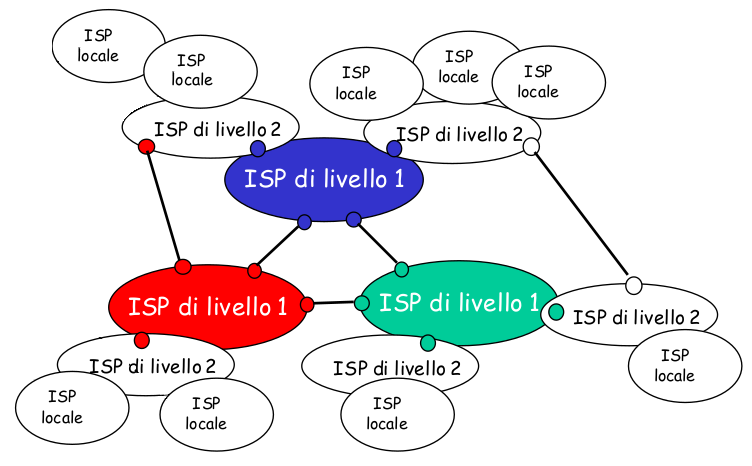
\includegraphics[scale=0.6]{introduzione-img17.png}
\end{center}

Come si pu\'o notare nella immagine precedente, con questa struttura gerarchica, si "stratifica" il livello del traffico, che 
raramente passa attraverso gli ISP T1, ma quasi sempre rimane confinato negli ISP T2, ad eccezione di necessit\'a particolari.

\subsection{Internet Protocol Suite}\label{internet-protocol-suite}
Sopra alla struttura fisica risiede il software di rete chiamato \textbf{IPS} \textit{(Internet Protocol Suite)}, ovvero 
l'implementazione del modello ISO/OSI per gestire la comunicazione tra host diversi, e potenzialmente, su reti diverse.

\paragraph{NB} \'E bene sottolineare che il modello di riferimento del software di rete ISO/OSI (sezione \ref{il-modello-iso-osi}) 
\underline{NON} \'e utilizzato in internet, in quanto viene usata la sua implementazione chiamata IPS basata su TCP/IP. Per questo 
motivo viene chiamato "modello" TCP/IP.

\begin{center}
	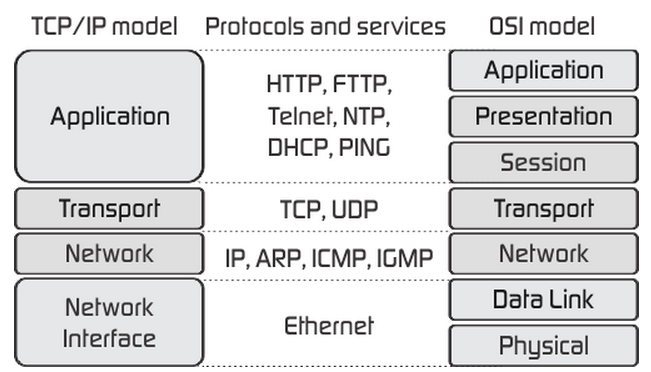
\includegraphics[scale=0.8]{introduzione-img18b.png}
\end{center}

Come si nota dall'immagine precedente, il modello e l'implementazione differiscono per molti livelli: il livello Fisico e 
Collegamento sono specificati pressoch\'e insieme, come il livello Applicazione, Presentazione e Sessione, perch\'e si riteneva 
inutile che il software di rete si occupasse di qualcosa che poteva prendersene cura l'applicazione stessa.

\clearpage
\subsubsection{IPS in breve}\label{ips-in-breve}
\begin{itemize}
	\item \textbf{Il livello Fisico o Network Interface} in IPS non venne specificato molto, pi\'u che un vero e proprio livello nel 
	senso usuale del termine \'e un'interfaccia tra l'host e il mezzo trasmissivo.
		
	\item \textbf{Il livello Internet o Network} \'e il perno che tiene insieme l'intera architettura. Il suo compito \'e permettere
	agli host di inviare pacchetti su qualsiasi rete e fare in modo che questi possano viaggiare indipendentemente verso la 
	destinazione. Potrebbero persino arrivare con un ordine diverso da quello con cui sono stati spediti, \'e compito del livelli 
	superiori riordinarli.
	
	Il livello Internet definisce un formato ufficiale per i pacchetti e un protocollo chiamato \textbf{IP} \textit{(Internet 	
	Protocolo)} accompagnato da un protocollo di supporto chiamato \textbf{ICMP} \textit{(Internet Control Message Protocol)}. Lo 	
	scopo del livello internet \'e quello di consegnare i pacchetti IP alla destinazione corretta.

	\item \textbf{Il livello Trasporto o Transport} \'e progettato per consentire la comunicazione end-to-end degli host sorgente e 
	destinazione, come il livello Trasporto in ISO/OSI. In questo livello sono stati definiti due protocolli: il primo, \textbf{TCP} 
	\textit{(Transmission Control Protocol)}, affidabile e orientato alla connessione che permette ad un flusso di byte emessi da un 
	computer di raggiungere senza errori qualsiasi altro computer in Internet.
	
	Il secondo protocollo di questo livello, \textbf{UDP} \textit{(User Datagram Protocol)} definisce uno standard di trasmissione 
	inaffidabile non orientato alla connessione per applicazioni che non vogliono la garanzia di ordinamento e controllo di flusso 
	di TCP, ma preferiscono gestire queste funzioni in modo autonomo.

	\item \textbf{Il livello Applicazione o Application} contiene tutti i protocolli di livello superiore: \textbf{SMTP} 
	\textit{(Simple Mail Transfer Protocol)}, \textbf{Telnet}, \textbf{FTP} \textit{(File Transfer Protocol)}, \textbf{DNS} 
	\textit{(Domain Name System)}, \textbf{HTTP} \textit{(Hyper Text Transfer Protocol)} ecc...
\end{itemize}



\end{document}
